\documentclass[12pt,a4paper]{article}
\usepackage[utf8]{inputenc}
\usepackage{amsmath}
\usepackage{amsfonts}
\usepackage{amssymb}
\usepackage{graphicx}
\usepackage[left=2cm,right=2cm,top=2cm,bottom=2cm]{geometry}
\author{leonardo}
\title{practica 3}
\begin{document}

Práctica 4: “activación de optocopladores”

\begin{document}


unidad de aprendizaje: transistores de efecto de campo.

objetivo: el alumno aprenderá a diseñar un puente h usando mosfet.

\section{material.
}

1.	Computadora
2.	Software para simulación de circuitos electrónicos.
3.	Fuente de voltaje regulable.
4.	Diodos de acción rápida.
5.	4 interruptores
6.	Protoboard
7.	JFET, 2N4220 o MOSFER IF540 / y su hoja de datos.
8.	Multímetro
9.	pulsos de reloj
10.	Motor de CD
11.	Flip-Flop tipo D (o un GAL programado como Flip-Flop)

\section{INTRODUCCIÓN}


El principio de utilizar un campo eléctrico para controlar el flujo de corriente se introdujo con el desarrollo del transistor BJT , por otro lado, los transistores de Efecto de Campo o Field Effect Transistores (FETs) es un dispositivo controlado por voltaje, estos son artefactos unipolares, o sea que en el proceso de conducción utilizan electrones o huecos y no ambos como los BJT.

El FET consiste de un semiconductor dopado (canal) con dos terminales en los extremos llamados Source y Drain. La corriente en el canal (entre Drain y Source) es controlada por el voltaje en un tercer terminal llamado Gate.
Los FETs se dividen en tres categorías principales:  el transistor de efecto de campo de unión (JFET), el transistor de efecto de campo semiconductor de óxido metálico (MOSFET), y el transistor de efecto de campo semiconductor metálico (MESFET). La categoría MOSFET se divide aún más en tipos de empobrecimiento y enriquecimiento.

El transistor MOSFET ha llegado a ser uno de los dispositivos más importantes utilizados en el diseño y construcción de circuitos integrados para computadoras digitales. Sin embargo, por ser un elemento discreto confinado en un contenedor acopado, requiere un manejo cuidadoso. El MESFET es un desarrollo más reciente y aprovecha al máximo la ventaja de las características de alta velocidad del GaAs como material semiconductor base. Aun cuando en la actualidad es la opción más cara, el tema del costo a menudo es superado por la necesidad de mayores velocidades en diseños de radiofrecuencia y de computadoras.


Al igual que los BJT, los FETs son interruptores de dos semirectas en el mismo cuadrante y, en consecuencia, con encendido y apagado controlados, pero se distinguen de éstos porque la corriente de salida está controlada por un voltaje. Las ventajas de los FETs con respecto a los BJT incluyen menos ruido, mayor estabilidad termal, mayor disipación de potencia y que pueden sostener corrientes muy altas, entre las desvantajas se encuentran una pobre respuesta de frecuencia debido a la alta capacitancia de entrada y a que se dañan fácilmente con la electricidad estática.

\section{PROCEDIMIENTO:
}

Se desea realizar una fuente de tensión reversible en corriente y voltaje con una fuente de voltaje
Esta consistirá en que por medio del puente H y un puente rectificador de diodos que rectifican la corriente pasara de voltaje positivo a negativo y viceversa de voltaje positivo a negativo invirtiendo así la onda dándole el giro al motor por medio de un pulsador de derecha a izquierda y de izquierda a derecha.


\section{Análisis:
}

Dada la naturaleza de las dos fuentes, será posible enlazarlas mediante el convertidor de puente completo E/I



\section{Diagrama 1
}

Cuando cerramos los interruptores S1 y S4 obtendremos las siguientes graficas

SW1	SW2	SW3	SW4



Cuando cerramos los interruptores S2 y S3 obtendremos las siguientes graficas
Y activando el S2 y el S4 obtendriamos

SW1	SW2	SW3	SW4


La bidireccionalidad de la tensión y de la corriente de la fuente de corriente hace que deba de contemplarse las tres configuraciones indicadas anteriormente.

Agrupando este comportamiento, se deduce que todos los semiconductores han de ser iguales, formados por tres semirrectas y bidireccionales en corriente.

SW1	SW2	SW3	SW4





Este interruptor es realizable mediante la asociación de un transistor en anti paralelo con un diodo. Resultando en consecuencia, el convertidor indicado en la siguiente figura.


\section{Desarrollo}

1.	Usando un simulador, arme el circuito de la Diagrama 1 sustituyendo la fuente de corriente por un medidor de corriente y de voltaje
2.	cierre los interruptores como se explicó en los procedimientos anteriores y observe como se ven afectados los medidores de corriente y voltaje y grafique
3.	Arme el diagrama 2 usando un flip-flop tipo D o un GAL preprogramada y un generador de pulsos

 
 
consideraciones para las conclusiones.

Unidad de aprendizaje: transistores de efecto de campo.

Objetivo: El Alumno aprenderá a controlar un foco por medio de transistores y optocopladores.

\section{Material:
}

1.	Computadora
2.	Software para simulación de circuitos electrónicos.
3.	Fuente de voltaje regulable.
4.	Diodos de acción rápida.
    5   Protoboard
    6   resistencia variable de 100k
7	optocopladores 4n25
    8   transistores n222A.
9   Multímetro
10  arduino uno
11   relay


\section{Desarrollo:
}

1.	Usando un simulador, arme el circuito de la Diagrama 1 sustituyendo la fuente de corriente por un medidor de corriente y de voltaje
2.	Conecte los optocopladores junto con las resistencias y los leds en serie cunto con el transistor n2222A como se explicó en los procedimientos anteriores y observe como se ven afectados los medidores de corriente y voltaje y grafique
3.	Arme el diagrama 2 usando los transistores de potencia para controlar el giro del foco dando 3 cantidades de iluminación diferentes.


\section{Conclusión:
}
en esta practica vemos como usando los mosfet como filtro de potencia vemos como podemos invertitr el giro del motor el cual esa funcion podemos usrla en diferentes aspectos por ejemplo la puerta del garage el cual podemos hacer que de un boton suba y que el otro baje ademas en otros aspectos como hacer que se valla una barra y regresa ademas vemos que la conexion es algo simple 

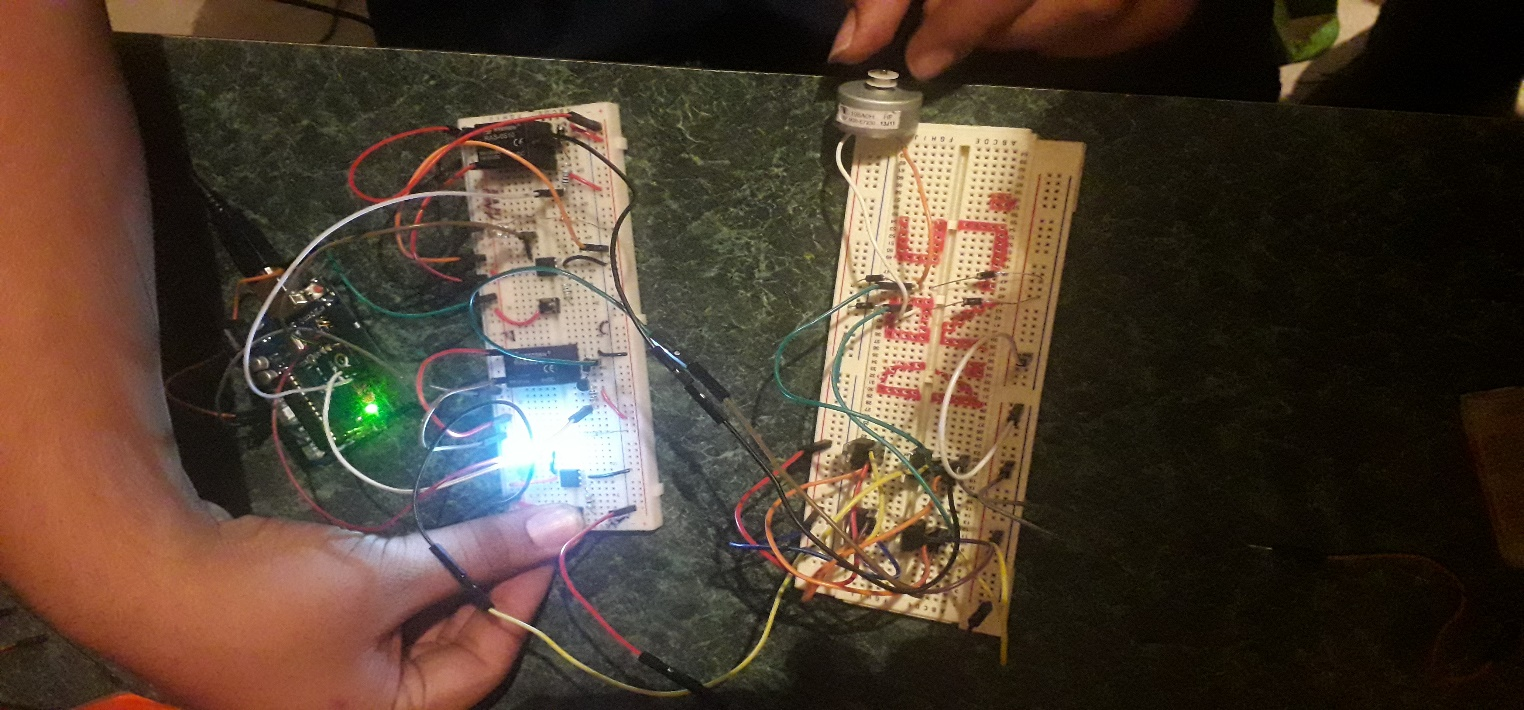
\includegraphics[width=10cm]{1.1.jpg} 





\end{document}